\documentclass{article}
\usepackage[utf8]{inputenc}

\title{Advanced Programming Labwork 10}
\author{Tom HERBRETEAU }
\date{November 2018}

\usepackage{natbib}
\usepackage{graphicx}
\usepackage{pgfplots}
\pgfplotsset{compat=newest}

\begin{document}

\maketitle
Every performance measures are done on ICT4 with eiffel.jpg, without counting the image saving.
\section{Introduction}
We have to apply the Kuwahara filter on the input image.
\section{Implementation}
I use to kernel to implement the kuwahara filter. The first one is HSV from lab 8 because kawahara need V the intensity of pixel. Then we define a region size, and apply the filter.
I use one kernel to compute all step of kuwahara, just one big MAP. 
Step 1 : initialize data for each region (could be optimized by a structure).
Step 2 : compute the average of V for each region, and the average of RGB (could be optimized by computing only the RBG average which be applied, because I compute average for each region, but only one of them is used finally, second way to optimized, compute V here instead of compute before, because we don't need H and S, and our HSV kernel isn't optimized).
Step 3 : compute the standard derivation for each region.
Step 4 : apply the result on output image.
To note i reduce the number of thread per block to 512 due to GPU's memory insufficiency when region became bigger.
\section{Result}    
Beautiful, of course.
The process time is exponential, depending on region size. For a region size of 8, the process last 273ms and it grows up faster when you choose region size like 32, 50 or 200 ! (to process a 250 pixel region size filter, it lasts 1336972.0ms (~22minutes))
\newline
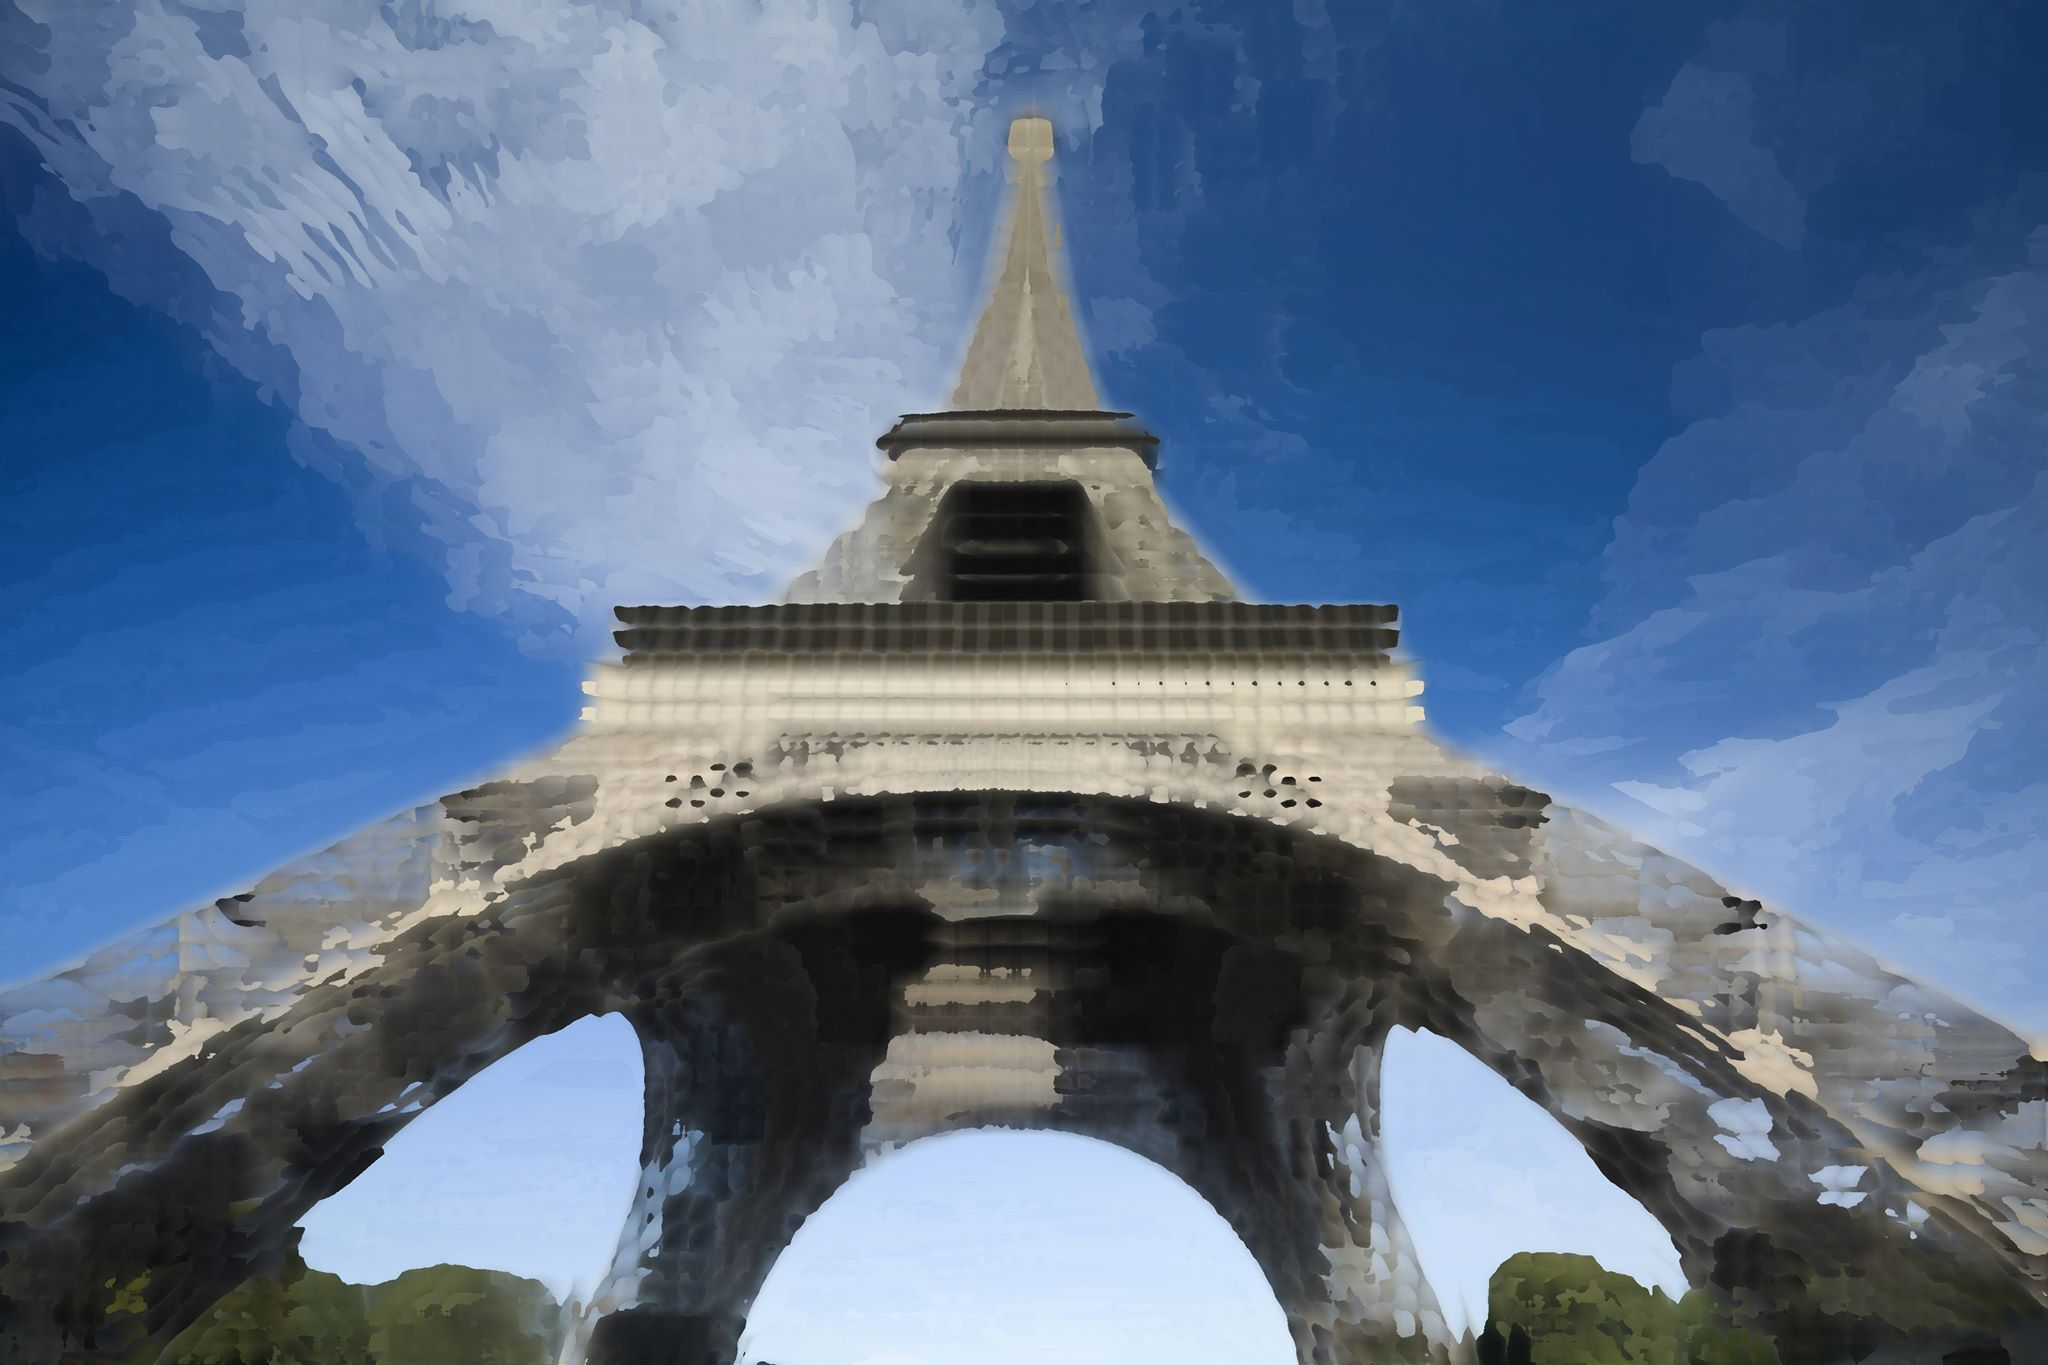
\includegraphics[width=\textwidth]{labwork10-gpu-out.jpg}
\newline
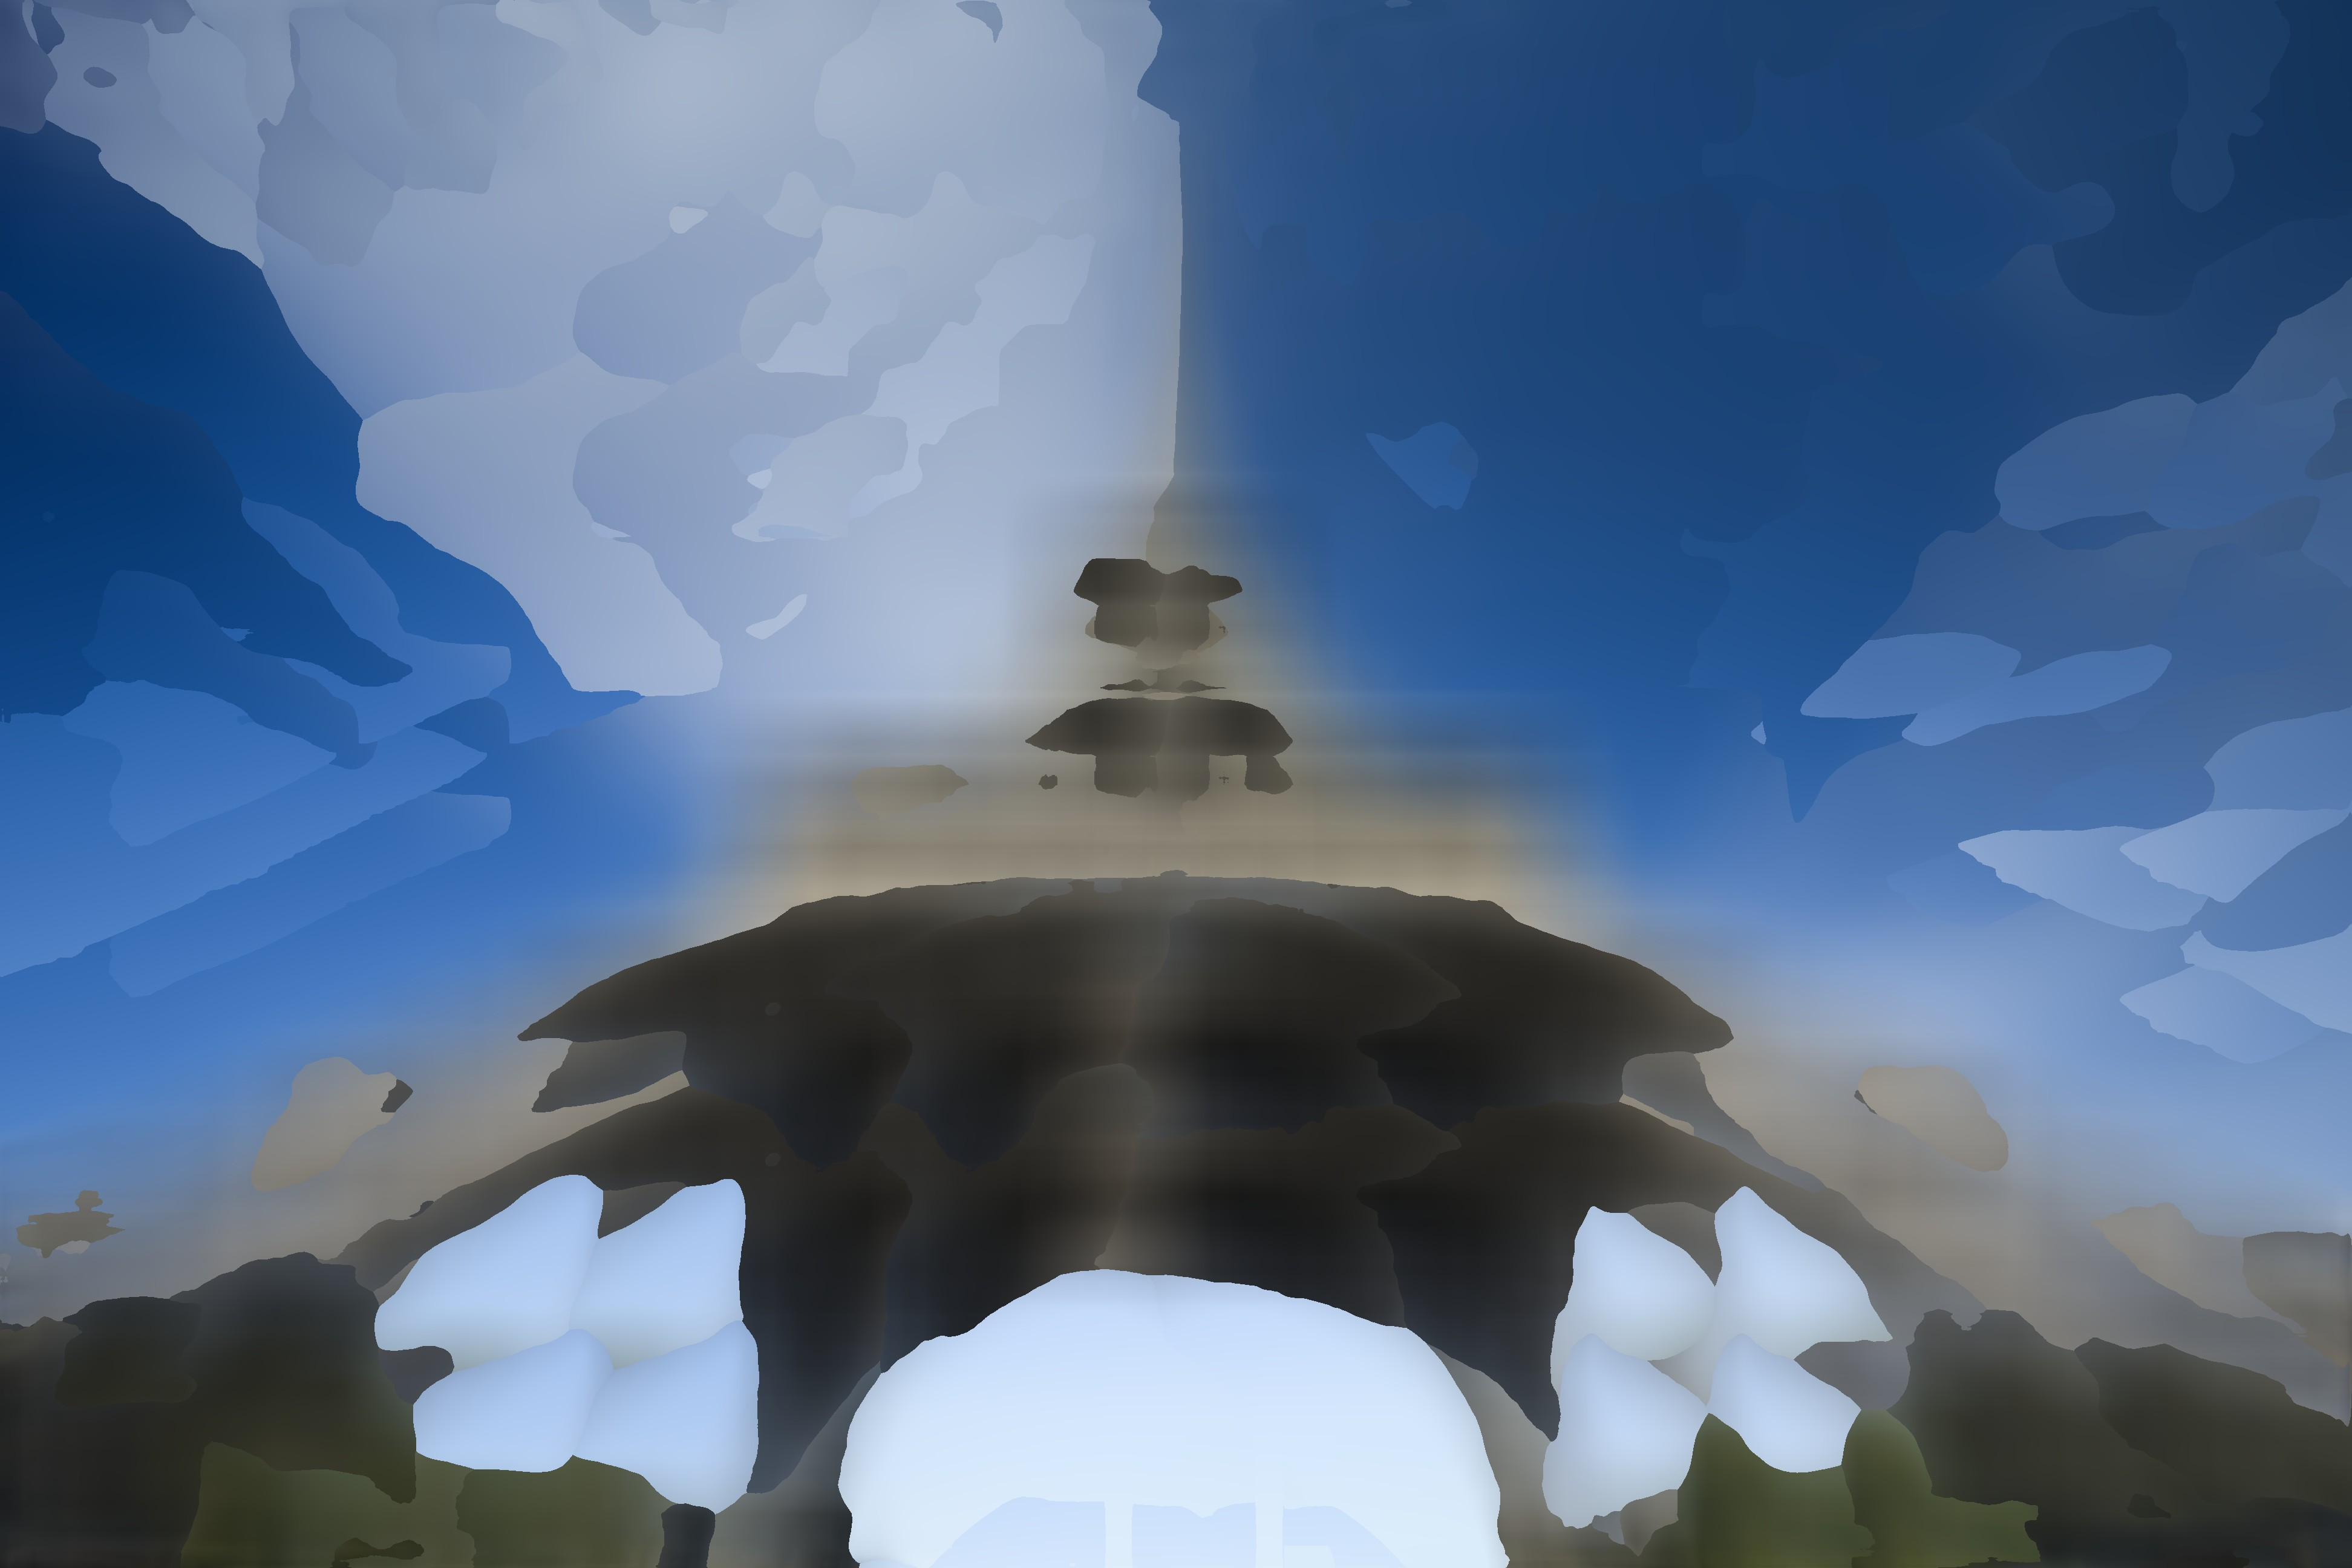
\includegraphics[width=\textwidth]{labwork10-gpu-out-250regionsize.jpg}
\bibliographystyle{plain}
\end{document}

